\documentclass[a4paper,11pt]{article}

\usepackage[utf8]{inputenc}
\usepackage[T1]{fontenc}
\usepackage{lmodern}

\usepackage[babel=true]{microtype}
\usepackage[portuguese]{babel}

\usepackage[newfloat]{minted}
\setminted{style=default}

\usepackage{spverbatim}

\usepackage{graphicx}
\usepackage{color}
\usepackage{listingsutf8}
\usepackage{array}
\usepackage{tabulary}
\usepackage{float}

\usepackage{hyperref}
\usepackage{indentfirst}
\usepackage{amsmath}
\usepackage{caption}
\usepackage{subcaption}



\usepackage{hyperref}
\hypersetup{
	colorlinks=true, %set true if you want colored links
	linktoc=all,     %set to all if you want both sections and subsections linked
	linkcolor=blue,  %choose some color if you want links to stand out
}

\begin{document}

\begin{titlepage}
\title{\huge \textbf{Pesquisa aplicada à gestão de projetos
\\[1cm]
\includegraphics{logo.png}\\[1cm] \large Inteligência Artificial\\[0.30cm] \normalsize $3^o$ ano $2^o$ semestre\\[0.05cm]Mestrado Integrado em Engenharia Informática e Computação\\[1cm]\textbf{Turma 5 - Grupo A1\_1}}}

\author{Hugo Drumond\\hugo.drumond@fe.up.pt\\ee11247 (up201102900)\\[1cm]}

\maketitle
\thispagestyle{empty} % titlepage must not be numbered

\end{titlepage}

\tableofcontents
\clearpage

\section{Objetivo}

Desenvolver um projeto sobre Pesquisa Sistemática e Informada de Soluções para Gestão de Projetos. Com a finalidade de determinar a melhor associação de elementos a uma equipa de projeto, maximizando o desempenho global. Mais concretamente a maximização da soma dos desempenhos das competências dos elementos na atribuição às tarefas de forma a reduzir o tempo total do projeto. Para alcançarmos tal, utilizou-se a seguinte estratégia:
\begin{itemize}
\item Implementação do algoritmo A*;
\item Visualização gráfica para debug da solução;
\item Preparação de diversos dados de input;
\item Colheita de dados para análise de resultados. De forma a verificar a qualidade da heurística vs Branch and Bound ($h = 0$) vs Default ($g = 0, h = 0$) (neste caso não é BFS (nem DFS) porque foi utilizado uma Fibonacci heap. A ordem após add não respeita nem append (BFS) nem prepend (DFS)).
\end{itemize}

\section{Especificação}	

\subsection{Descrição}

``A alocação dos elementos mais adequados a um projeto é essencial para o seu sucesso. Um projeto é constituído por um conjunto de tarefas a desenvolver por um ou mais elementos. As tarefas podem ter precedências entre si e têm uma duração (pessoa/mês). Cada elemento candidato possui um conjunto de competências, que permitem satisfazer uma ou mais tarefas. É conhecido ainda o desempenho (valor de 1 a 5) de um elemento em cada uma das suas competências. O trabalho consiste em determinar a melhor alocação de elementos às várias tarefas de um projeto de modo a maximizar o desempenho global. Um elemento não pode estar alocado a mais que uma tarefa ao mesmo tempo.''

\subsection{Análise do Problema}

O problema tem como inputs:
\begin{itemize}
	\item Tarefas. Cada qual com:
	\begin{itemize}
		\item Precedências;
		\item Duração;
		\item Competências necessárias.
	\end{itemize}
	\item Elementos. Cada qual com:
	\begin{itemize}
		\item Competências. Cada qual com:
			\begin{itemize}
				\item Pares, Competência-Desempenho, com Desempenho compreendido entre 1 a 5.
			\end{itemize} 
	\end{itemize}	
\end{itemize}

Existem algumas restrições inerentes ao problema, nomeadamente:
\begin{itemize}
	\item Um elemento não pode estar alocado a mais que uma tarefa ao mesmo tempo;
	\item Um elemento tem de conter todas as competências necessárias para efetuar uma tarefa;
	\item Uma tarefa só pode ser atribuída após as suas precedências terem sido efetuadas;
	\item As precedências de tarefas têm de ser acíclicas (têm de ser um DAG).
\end{itemize}

\begin{figure}[H]
	\centering
	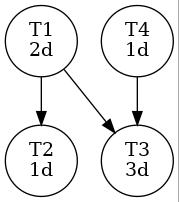
\includegraphics[scale=0.4]{tasks_graph.jpeg}
	\caption{Exemplo de Grafo acíclico de Tasks}
	\label{fig:tasks_graph}
\end{figure}

O programa analisa estes dados e determina que elementos atribuir a cada tarefa respeitando as restrições do problema. A dificuldade está, portanto, em modelar todas as características do problema: competências, tarefas, precedências, compatibilidade de combinações de elementos, duração, etc de um modo eficiente (em espaço e tempo). A solução final deverá maximizar o desempenho global, que corresponde à alocação ótima dos vários elementos às várias tarefas de forma a minimizar o tempo total do projeto.

\subsubsection{Cenários}

A alocação de um elemento com muitas competências a uma tarefa simples (com poucas competências) quando esta poderia ter sido atribuída a um elemento mais restrito poderá bloquear a execução em paralelo de tarefas mais complexas. Aumentando assim a duração do projeto.\\

A escolha de um elemento muito polivalente para uma tarefa simples longa quando esta poderia ter sido atribuída a um elemento com um conjunto de competências mais restrito poderá bloquear a execução de tarefas até que o elemento polivalente esteja novamente disponível.\\

Não será possível encontrar uma solução caso haja pelo menos uma tarefa que necessite de competências que nenhum dos elementos possui.\\

É possível esperar pela disponibilidade de mais elementos para então começar uma tarefa.

\subsubsection{Representação do Conhecimento}

A informação sobre as tarefas e elementos, e todas as suas características, é capturada de ficheiros JSON com a seguinte estrutura:

\begingroup
\inputminted[breaklines=false,fontsize=\footnotesize]{json}{exemplo_input.json}
\captionsetup{type=figure}
\captionof{listing}{Ficheiro de input exemplo JSON}
\endgroup
\subsection{Abordagem}

O algoritmo A* resulta da combinação do algoritmo branch and bound ($g$) e greedy ($h$), ou seja, soma dos custos acumulados e estimativas do custo até à solução (deverá ser otimista). $f(n) = g(n) + h(n)$. Para garantir que se chega à solução ótima é necessário que a heurística seja consistente, $h(x) <= d(x, y) + h(y)$ (monótona).

\subsubsection{Estados}
Utilizou-se a seguinte representação para o estado:
\begin{minted}[breaklines]{java}
private PersistentHashSet<Task> remainingTasks;
private PersistentHashSet<Element> elementsNeverAllocated;
private PersistentHashSet<Element> elementsBeenAllocated;
private PersistentHashMap<Task, Integer> taskPrecedencesCounter;
private PersistentHashMap<Integer, TaskResult> taskIdTaskResult;
private PersistentTreeMap<Double, PersistentVector<TaskResult>> startTimeTaskResult;
private double maxEndTime = 0;
\end{minted}

Foram usadas estruturas de dados persistentes de modo a: evitar desperdícios de memória e facilitar a gestão dos dados na geração de novos estados (evitar partilhas de dados não desejadas, problemas com clones). O estado inicial é:

\begin{minted}[breaklines]{java}
State state = new State();

state.remainingTasks = PersistentHashSet.of(problemData.getTasks());

state.elementsNeverAllocated = PersistentHashSet.of(problemData.getElements());

PersistentHashMap.MutableHashMap<Task, Integer> taskPrecedencesCounterMut = PersistentHashMap.emptyMutable();
for (Task task : problemData.getTasks()) {
	taskPrecedencesCounterMut.assoc(task, task.getPrecedences().size());
}
state.taskPrecedencesCounter = taskPrecedencesCounterMut.immutable();

state.elementsBeenAllocated = PersistentHashSet.empty();

state.taskIdTaskResult = PersistentHashMap.empty();

state.startTimeTaskResult = PersistentTreeMap.empty();
\end{minted}

As variáveis \textit{remainingTasks}, \textit{elementsNeverAllocated} e \textit{taskPrecedencesCounter} foram inicializadas com, respetivamente: todas tarefas do problema, elementos do problema, contabilidade de precedências para cada tarefa. É encontrada uma solução possível quando \textit{state.remainingTasks.size == 0}. 

\subsubsection{Função de Transição}

Cada novo estado gerado é resultado da atribuição de um dado conjunto de elementos a uma dada tarefa que agora já não tem precedências.

\begin{minted}[breaklines]{java}
public ImmutableList<State> generateSuccessors() {

	ImmutableList<Task> tasksCurrentlyWithNoPrecedences = pickTasksCurrentlyWithNoPrecedences();

	ImmutableList.Builder<State> successorsStatesBuilder = new ImmutableList.Builder<>();

	for (Task selectedTask : tasksCurrentlyWithNoPrecedences) {
		ImmutableList<ElementsCombination> elementsCombinations = getCompatibleElementsCombinations(selectedTask);
		
		generateNewStates(selectedTask, elementsCombinations, successorsStatesBuilder);
	}

	return successorsStatesBuilder.build();
}
\end{minted}

A função \textit{pickTasksCurrentlyWithNoPrecedences()} retorna as tarefas que neste estado já não têm precedências. Para cada tarefa são encontradas todas as combinações de elementos compatíveis, \textit{getCompatibleElementsCombinations}. Uma combinação, \textit{ElementsCombination} possui a seguinte informação:\newpage

\begin{minted}[breaklines]{java}
private static class ElementsCombination {
	private final double startTime;
	private final double duration;
	private final ImmutableSet<Element> elements;
	private final PersistentHashSet<Element> elementsNeverAllocated;
	private final PersistentHashSet<Element> elementsBeenAllocated;
}
\end{minted}

O tempo de começo (\textit{starTime}) e duração (\textit{duration}) dependem, respetivamente, de:
\begin{itemize}
	\item disponibilidade de cada elemento (aguardar por todos do conjunto \textit{elements}) e a sua precedência que termina mais tarde
	\item valores das competências de cada um (só para $task.skills$)
\end{itemize}

A duração de cada tarefa é dada por:
\[
\frac{T}{\sqrt{m_K + ...}}
\]

Em que $T$ representa a duração da tarefa a atribuir e $m_K$ a média dos valores das competências do elemento $K$ que são utilizadas nesta tarefa.\\

\textit{getCompatibleElementsCombinations} trata de chamar a função \textit{getStartTime} que faz shifts da range \textit{[startTime, startTime+duration]} (\textit{starTime} começa com \textit{endTime} da sua precedência que acaba mais tarde) e intercepta com ranges das tarefas já alocadas e seus elementos de modo a encontrar uma range válida (usa o \textit{TreeMap} \textit{startTimeTaskResult}).\\
 
As variáveis \textit{elementsNeverAllocated} e \textit{elementsBeenAllocated} representam a nova configuração de elementos não alocados e alocados para o novo estado a ser gerado a partir desta combinação.\\

A lista de combinações, \textit{ImmutableList<ElementsCombination>}, é então passada para \textit{generateNewStates} onde é criado um estado para cada ElementsCombination com \textit{remainingTasks}, \textit{elementsNeverAllocated}, \textit{elementsBeenAllocated}, \textit{taskPrecedencesCounter}, \textit{taskIdTaskResult}, \textit{startTimeTaskResult}, \textit{maxEndTime} atualizados.

\subsubsection{Função de custo}

O custo acumulado representa o impacto de não se conseguir fazer uma tarefa em paralelo. É dado por:
\begin{minted}[breaklines]{java}
double getTotalTimeDelta(State destinationState) {
	return destinationState.maxEndTime - maxEndTime;
}
\end{minted}

O custo posterior foi calculado pegando na tarefa atualmente sem precedências com o maior endTime assumindo que todos os elementos estão disponíveis.
\begin{minted}[breaklines]{java}
double heuristic() {
	double taskMaxEndTime = maxEndTime;
	for (Task task : pickTasksCurrentlyWithNoPrecedences()) {
		double startTime = getTaskStartTimeFromPrecedences(task);
		double elementsCompetenceSum = getCompatibleElementsSum(task);
		double duration = getTaskReducedDuration(task.getDuration(), elementsCompetenceSum);
		taskMaxEndTime = Math.max(taskMaxEndTime, startTime + duration);
	}
	return taskMaxEndTime - maxEndTime;
}
\end{minted}

A heurística presente no relatório intercalar: resolução do problema relaxado por remoção da restrição de um elemento não poder estar alocado a mais que uma tarefa ao mesmo tempo, respeitando as precedências; revelou ser demasiado complexa piorando o tempo de execução. Portanto, foi desprezada.

\section{Desenvolvimento}
Utilizou-se a linguagem de programação Java para a codificação do algoritmo; e Javascript para criar a interface de visualização. Foi usado o sistema de compilação Gradle. As bibliotecas Java usadas foram:
\begin{itemize}
	\item com.google.code.gson:gson — deserializar e serializar JSON
	\item org.graphstream:gs-algo — fibonacci heap
	\item com.google.guava:guava — ranges e coleções imutáveis
	\item org.organicdesign:Paguro — coleções persistentes
\end{itemize}

Para executar o programa basta ter o gradle instalado e correr \mintinline[breaklines]{bash}{gradle run -Pargs="../data/1a.json"} na pasta \textit{project\_management}. Os ficheiros resultado são colocados na mesma pasta que o input \mintinline[breaklines]{bash}{"../data/1a_{{algo}}.json"}.

Para visualizar a solução é necessário abrir o ficheiro \textit{index.html}, pasta \textit{web\_visualizer}, e importar, por exemplo, 1a.json e 1a\_astar.json.

\subsection{Arquitetura da aplicação}

\begin{figure}[H]
	\centering
	\makebox[\textwidth][c]{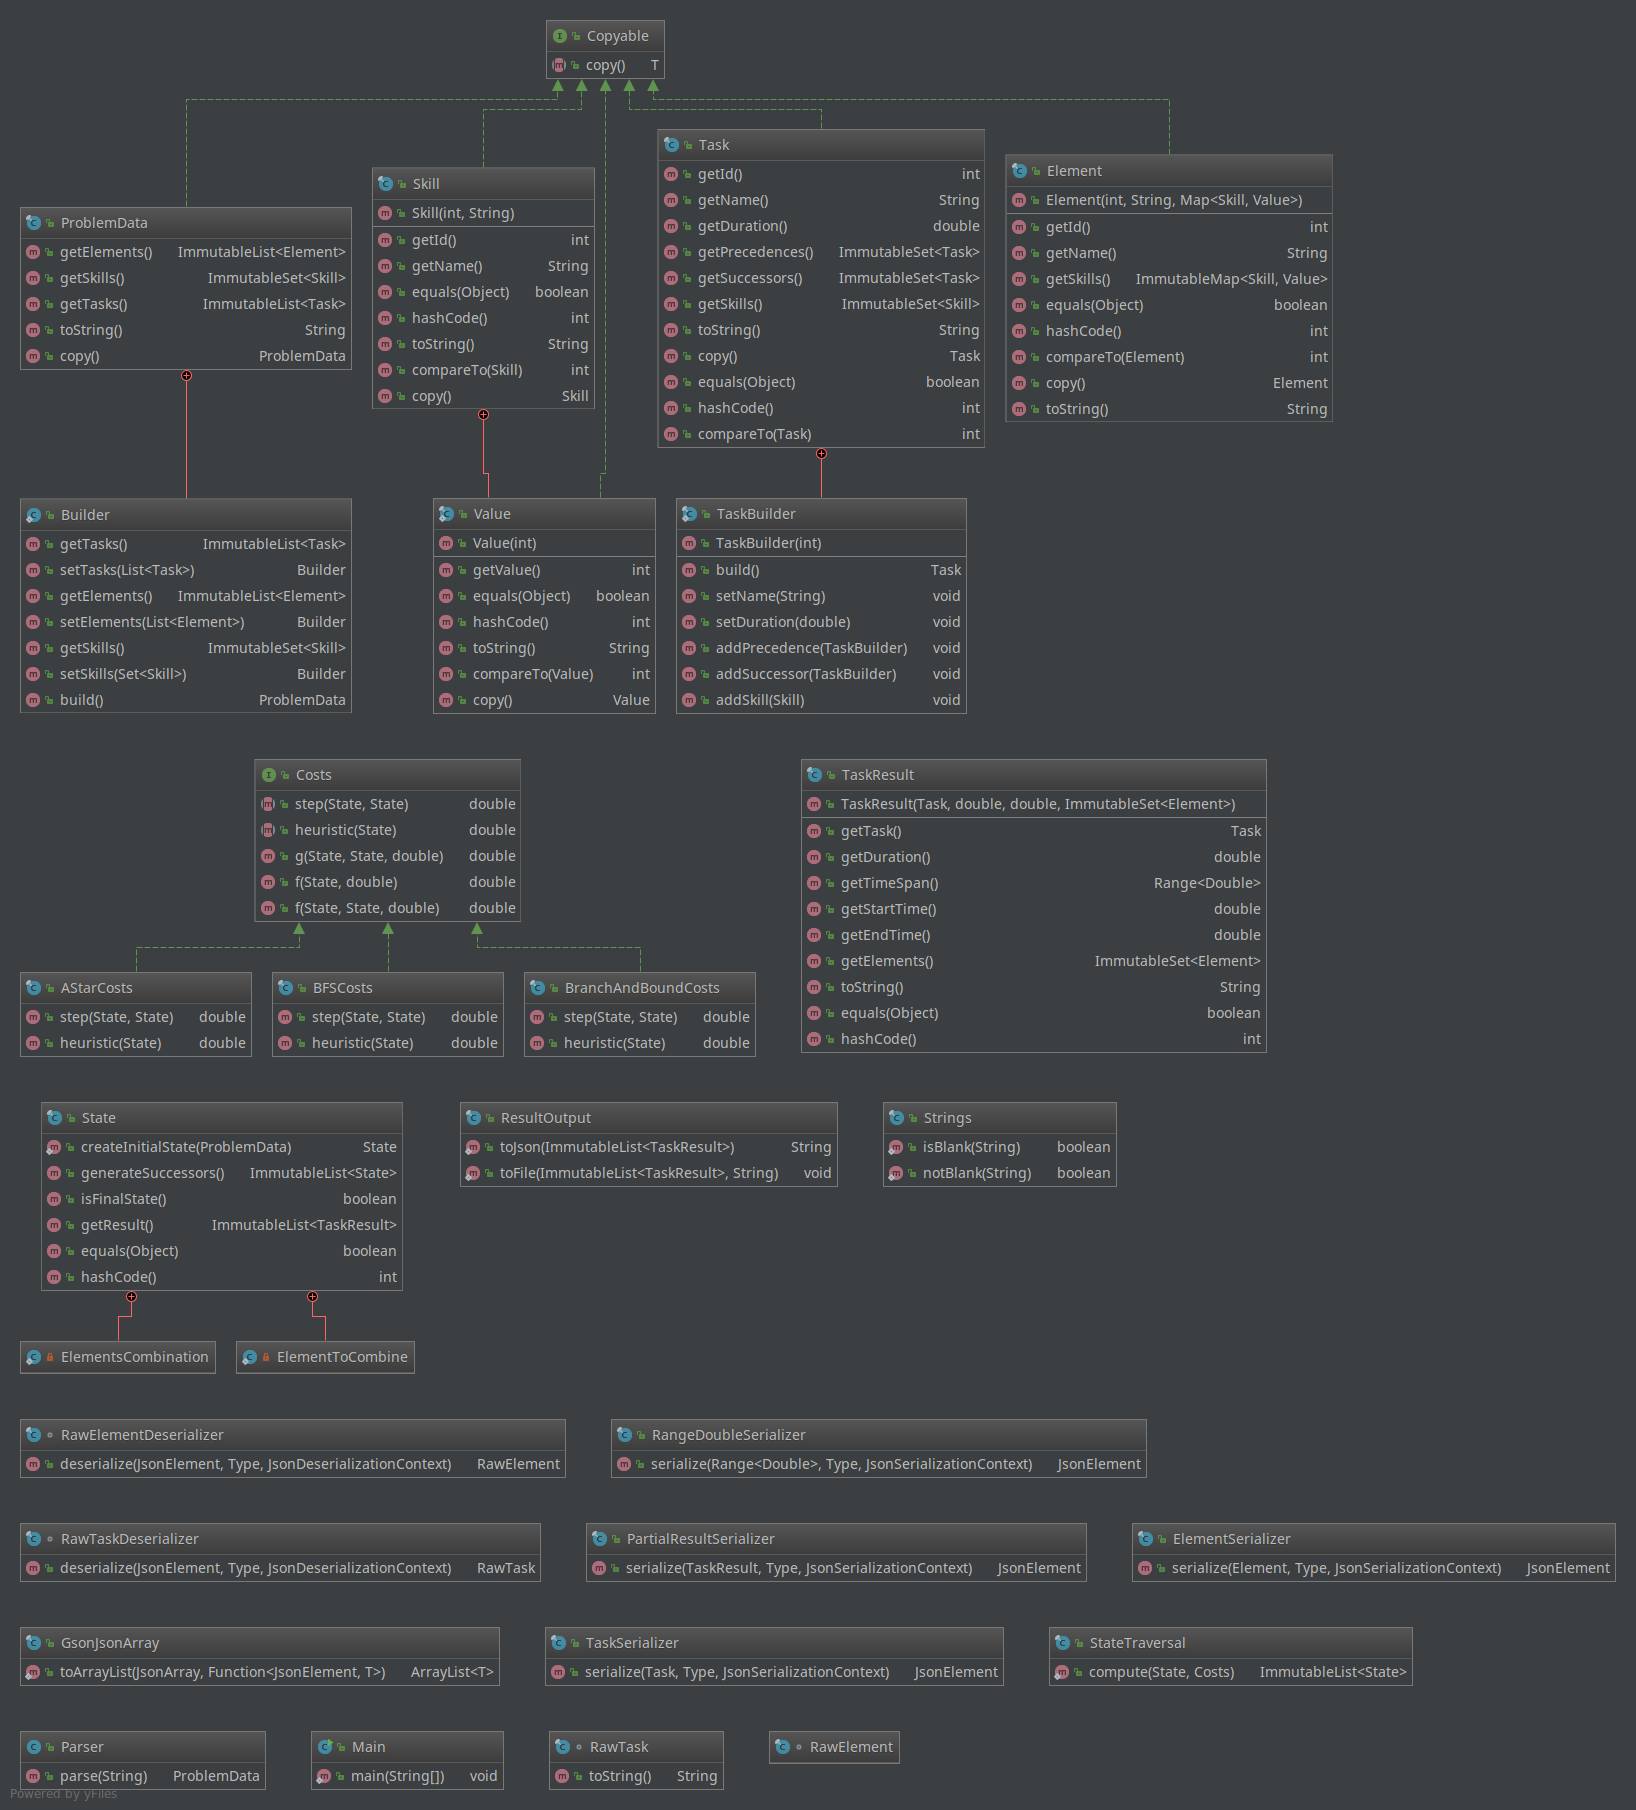
\includegraphics[width=1.25\textwidth]{classes.png}}
	\caption{Project Classes (only public methods)}
	\label{fig:classes}
\end{figure}

\begin{figure}[H]
	\centering
	\makebox[\textwidth][c]{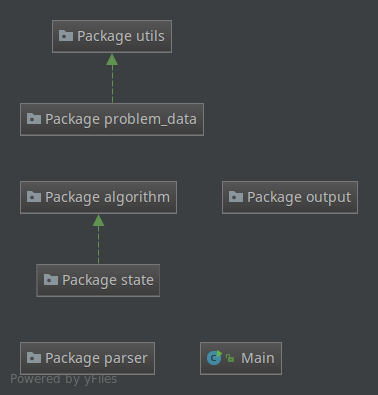
\includegraphics[width=0.5\textwidth]{packages.png}}
	\caption{Project Packages}
	\label{fig:packages}
\end{figure}

\subsection{Detalhes Relevantes da implementação}

Foi tido em atenção as complexidades espaciais e temporais da implementação, respetivamente, estruturas de dados persistentes e Fibonacci Heap (decreaseKey, O(1) amortized running time, atualização gScores da openList).

\section{Experiências}
A validação dos resultados é feita através da visualização gráfica de uma timeline presente numa página web. São usados vários datasets com diferentes dimensões e topologias de forma a melhor compreender o comportamento do algoritmo A* vs Branch and Bound vs Default. No início do projeto foram usados ficheiros de input relativamente pequenos de modo a confirmar a boa operação do programa. Numa fase posterior foram realizados testes de dimensão média. Os tempos foram calculados a partir da média de amostras de dimensão 5 (outliers desprezados).

\subsection{Resultados das Experiências}
\subsubsection{Experiência 1a.json}

Tarefas com precedências, elementos com conjunto de competências diferentes.

\begin{center}
	\begin{tabular}{|c|c|c|} 
		\hline
		\multicolumn{3}{|c|}{Time (microseconds)} \\
		\hline
		Default & B\&B & $A^*$\\
		\hline
		29416 & 49164 & 47223\\
		\hline
	\end{tabular}
\end{center}

\subsubsection{Experiência 1b.json}

Tarefas sem precedências, elementos com conjunto de competências diferentes.

\begin{center}
	\begin{tabular}{|c|c|c|} 
		\hline
		\multicolumn{3}{|c|}{Time (microseconds)}\\
		\hline
		Default & B\&B & $A^*$\\
		\hline
		34413 & 72616 & 74578\\
		\hline
	\end{tabular}
\end{center}

\subsubsection{Experiência 2a.json}

Tarefas com precedências, elementos com conjunto de competências igual.

\begin{center}
	\begin{tabular}{|c|c|c|} 
		\hline
		\multicolumn{3}{|c|}{Time (microseconds)} \\
		\hline
		Default & B\&B & $A^*$\\
		\hline
		30111 & 57619 & 52724\\
		\hline
	\end{tabular}
\end{center}

\subsubsection{Experiência 2b.json}

Tarefas sem precedências, elementos com conjunto de competências igual.

\begin{center}
	\begin{tabular}{|c|c|c|} 
		\hline
		\multicolumn{3}{|c|}{Time (microseconds)} \\
		\hline
		Default & B\&B & $A^*$\\
		\hline
		43403 & 883716 & 902495\\
		\hline
	\end{tabular}
\end{center}

\subsubsection{Experiência 3a.json}

Tarefas com precedências, elementos com conjunto de competências igual e diferente.

\begin{center}
	\begin{tabular}{|c|c|c|} 
		\hline
		\multicolumn{3}{|c|}{Time (microseconds)} \\
		\hline
		Default & B\&B & $A^*$\\
		\hline
		39130 & 448284 & 312086\\
		\hline
	\end{tabular}
\end{center}

\subsubsection{Experiência 3b.json}

Tarefas sem precedências, elementos com conjunto de competências igual e diferente.

\begin{center}
	\begin{tabular}{|c|c|c|} 
		\hline
		\multicolumn{3}{|c|}{Time (microseconds)} \\
		\hline
		Default & B\&B & $A^*$\\
		\hline
		56205 & 5542214 & 5254838\\
		\hline
	\end{tabular}
\end{center}

\subsection{Análise heurística}

O algoritmo com Default ($g = 0, h = 0$) é o mais rápido visto não encontrar a solução ótima (neste caso não é BFS (nem DFS) porque foi utilizado uma Fibonacci heap. A ordem após add não respeita nem append (BFS) nem prepend (DFS)). Neste problema, o BFS também não encontraria a solução ótimo visto todas as soluções estarem no mesmo nível.

O Branch and Bound e $A^*$ (heurística consistente) encontram sempre a melhor solução. Para tarefas com precedências a heurística é tanto melhor quanto maior for a dimensão do problema.

\subsection{Visualização exemplo, experiência 1a.json}

\begin{figure}[H]
	\centering
	\makebox[\textwidth][c]{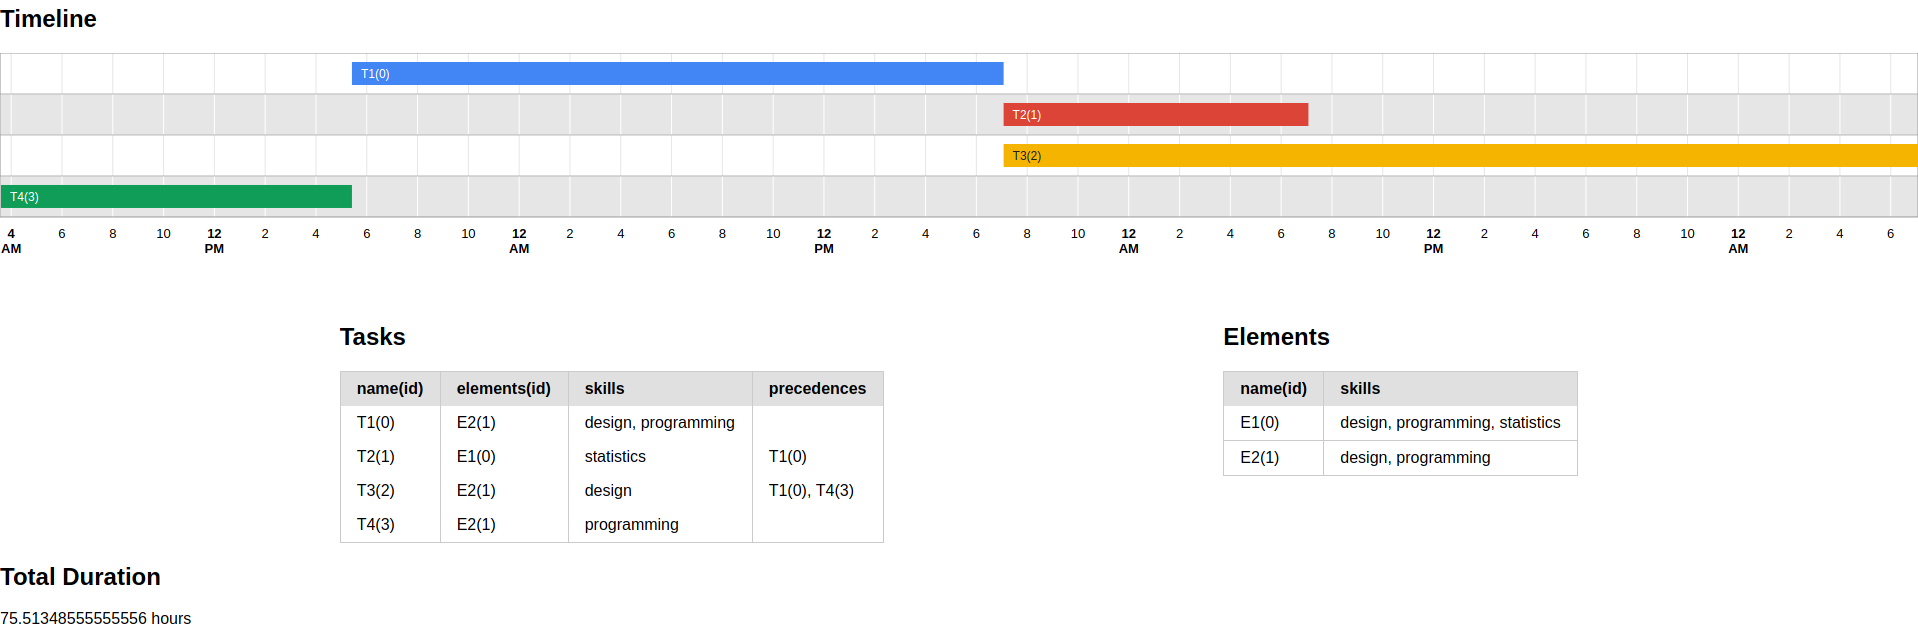
\includegraphics[width=1.45\textwidth]{1a_default.png}}
	\caption{Visualização 1a.json, 1a\_default.json}
	\label{fig:1adefault}
\end{figure}

\begin{figure}[H]
	\centering
	\makebox[\textwidth][c]{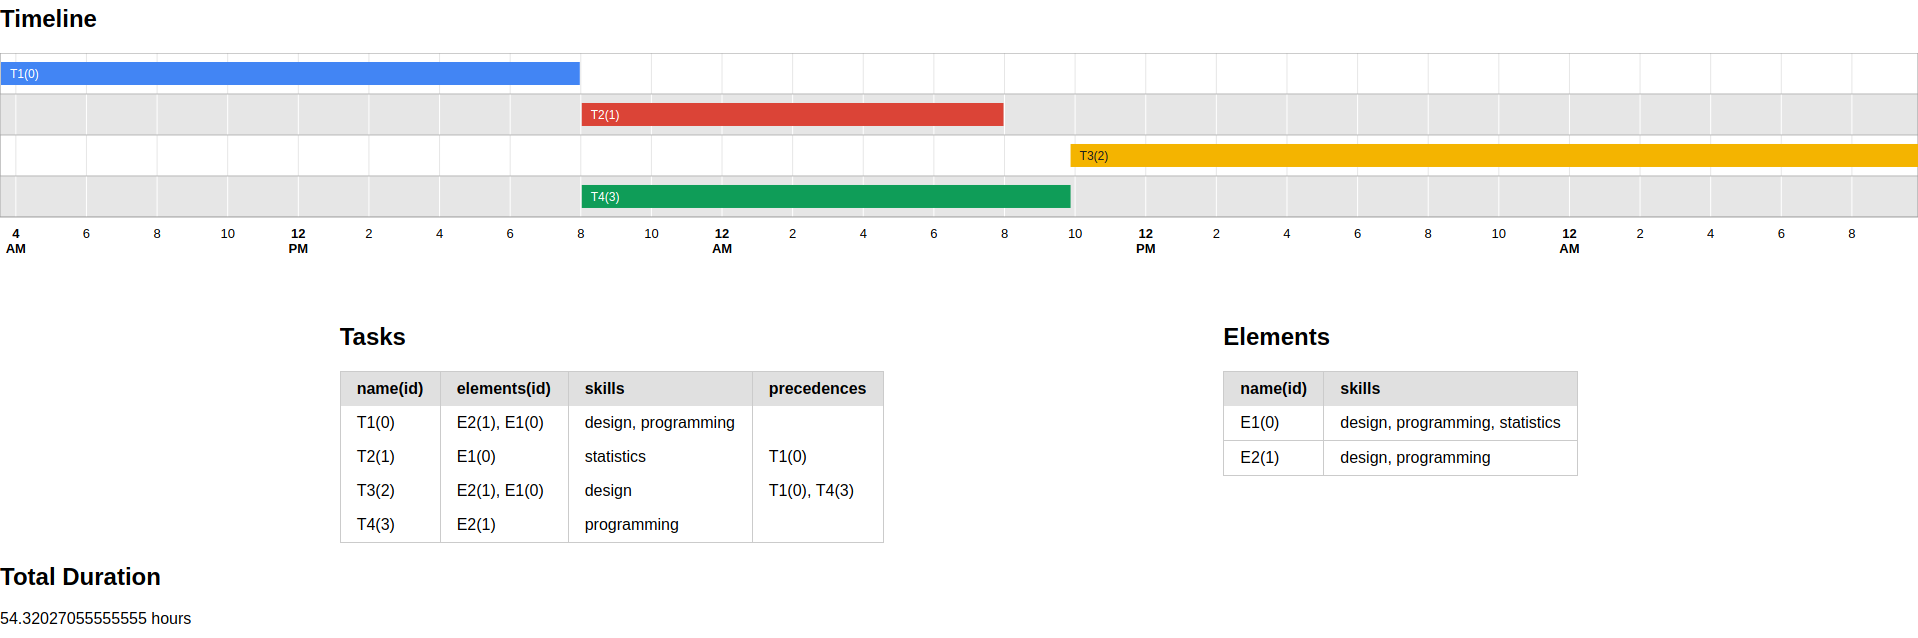
\includegraphics[width=1.45\textwidth]{1a_astar.png}}
	\caption{Visualização 1a.json, 1a\_astar.json}
	\label{fig:1aastar}
\end{figure}

\section{Conclusões}

Chegou-se à conclusão que a dificuldade nestes algoritmos centra-se na modelação do problema (estados, função de transição, ações, custos) e na descoberta de uma heurística não muito complexa que garanta o resultado ótimo (consistente) em menor tempo. Como era de prever o Branch and Bound e o $A^*$ (visto a nossa heurística ser consistente) encontram a solução ótima. A heurística discriminada no relatório intercalar (sem dados de experiências presentes) era pior que o Branch and Bound em todos os casos testados. Ou seja, a heurística era demasiado complexa. A nova, descrita com pormenor no relatório, apresenta dados temporais semelhantes ao Branch and Bound quando as tarefas não têm precedências (1b, 2b, 3b). No entanto, para tarefas com precedências, a heurística é tanto melhor quanto maior for a dimensão do problema (1a, 2a, 3a).

\section{Melhoramentos}

Um possível melhoramento seria construir um gerador de estados mais inteligente que eliminasse combinações de elementos que se sabe à partida não poderem levar à solução ótima. Removendo assim o número excessivo de estados. Uma tarefa com $N$ elementos compatíveis tem $\sum {N \choose k} - 1, k \in [1, N] = 2^N - 1$ combinações destes (power set - conjunto vazio). Seria também útil fazer um estudo comparativo entre várias heurísticas, visto umas serem melhores para projetos de planeamento com diferentes topologias. Poderiam também ser introduzidas outras restrições como tempo máximo de trabalho por semana. Outro cenário que não foi contabilizado é a atribuição de um elemento a uma tarefa quando esta já está em execução.

\section{Recursos}
\subsection{Websites}
\begin{itemize}
	\item \href{https://paginas.fe.up.pt/~eol/IA/1718/ia_.html}{Slides das teóricas}
	\item \href{https://edge.edx.org/courses/course-v1:BerkeleyX+CS188+2018_SP/20021a0a32d14a31b087db8d4bb582fd/}{Artificial Intelligence - Berkeley (Spring 2018)}
	\item \href{http://theory.stanford.edu/~amitp/GameProgramming/}{Amit’s A* Pages From Red Blob Games}
\end{itemize}
\subsection{Software}
\begin{itemize}
	\item \href{https://www.jetbrains.com/idea/}{Intellij IDEA}
	\item \href{http://graphstream-project.org/}{GraphStream}
	\item \href{https://gradle.org/}{Gradle}
	\item \href{https://github.com/GlenKPeterson/Paguro}{Paguro}
	\item \href{https://github.com/google/gson}{Gson}
	\item \href{https://developers.google.com/chart/}{Google Charts}
	\item \href{https://github.com/pure-css/pure}{pure-css}
	\item \href{https://github.com/lodash/lodash}{lodash}
	\item \href{https://github.com/wycats/handlebars.js/}{handlebars}
\end{itemize}

\clearpage
\appendix

%\section{Manual do Utilizador}

\end{document}
